\documentclass{article}
\usepackage[a4paper, left=15mm, top=20mm, right=15mm,bottom=20mm]{geometry}
\usepackage{amsmath, amssymb, amsfonts}
\usepackage{fancyhdr}
\usepackage{graphicx}
\graphicspath{ {./images/} }
\usepackage{float}
\usepackage{hyperref}
\usepackage{lscape}
\usepackage{mathtools}

\pagestyle{fancy}
\fancyhf{}
\lhead{DSA2101}
\rhead{claudeonrs}
\rfoot{\thepage}
\usepackage{amsmath, amssymb, amsfonts, listings}
\usepackage{xcolor}
\usepackage{enumitem}
\setlist[itemize]{noitemsep, topsep=0pt}
\setlist[enumerate]{noitemsep, topsep=0pt}
\setlist[description]{noitemsep, topsep=0pt}


%New colors defined below
\definecolor{codegreen}{rgb}{0,0.6,0.4}
\definecolor{codegray}{rgb}{0.5,0.5,0.5}
\definecolor{codepurple}{rgb}{0.58,0,0.82}
\definecolor{backcolour}{rgb}{0.95,0.95,0.92}
\definecolor{commentgreen}{rgb}{0.4,0.8,0.6}
%Code listing style named "mystyle"
\lstdefinestyle{mystyle}{
  backgroundcolor=\color{backcolour},
  commentstyle=\color{red},
  keywordstyle=\color{blue},
  numberstyle=\tiny\color{codegray},
  stringstyle=\color{codegreen},
  basicstyle=\ttfamily,
  breakatwhitespace=false,
  breaklines=true,
  captionpos=b,
  keepspaces=true,
  numbers=left,
  numbersep=5pt,
  showspaces=false,
  showstringspaces=false,
  showtabs=false,
  tabsize=2
}

%"mystyle" code listing set
\lstset{style=mystyle}

\title{No Title}
\author{Claudeon R Susanto}
\date{}
\usepackage[T1]{fontenc}
\usepackage[utf8]{inputenc}
\usepackage[english]{babel}
\usepackage{lmodern}

\renewcommand{\familydefault}{\sfdefault}   % Supprime le serif (dyslexie)
\usepackage[font=sf, labelfont={sf}]{caption}
\usepackage{multicol}
\usepackage{makecell}
\renewcommand\theadalign{bc}
\renewcommand\theadfont{\bfseries}
\renewcommand\theadgape{\Gape[4pt]}
\renewcommand\cellgape{\Gape[4pt]}



% own commands
\newcommand{\eg}[0]{\textit{e.g. }}
\newcommand{\ie}[0]{\textit{i.e. }}
\newcommand{\impt}[0]{\textcolor{red}{\textbf{[IMPT] }}}


\renewcommand\thesubsection{\thesection.\arabic{subsection}}
\setlength{\columnseprule}{1pt}
\begin{document}
%\maketitle
\fontfamily{lmss}\selectfont
\begin{multicols}{2}
\section{R Programming}
\subsection*{List}
\begin{itemize}
	\item \texttt{[[idx]]}: get element in a list
	\item \texttt{str(ls)}: get \textbf{str}ucture of a list (similar to summary)
	\item \texttt{saveRDS} and \texttt{loadRDS}
	\item \texttt{unlist}: convert list to vector \impt
\end{itemize}
\subsection*{Recycling Rule}
\begin{itemize}
	\item shorter vectors are recycled until they match the length of the longest vector
	\item the length of the longest vector must be a multiple of the shorter vector in arithmetic operations!
\end{itemize}
\subsection*{Useful functions}
\begin{itemize}
	\item \texttt{sample(x, size, replace, prob)}
	\begin{itemize}
		\item \texttt{size}: length of output vector
		\item \texttt{replace}: if \texttt{TRUE}, then sampling is with replacement
		\item \texttt{prob}: a vector of probability weights
	\end{itemize}
	\item \texttt{any(duplicated(vec))}: returns true or false if there are any duplicated elements in a vector
	\item \texttt{rep(x, times, length.out)}
	\item \texttt{table()}
	\item \texttt{args(func)}: list the arguments of a function
	\item \texttt{seq(from, to, by, length)}
	\item \texttt{paste(v1, v2, sep)}: concatenate vectors after converting them to characters
	\begin{itemize}
		\item \texttt{sep}: separator between elements of \texttt{v1} and \texttt{v2}
		\item The recycling rule applies when \texttt{length(v1) != length(v2)}
	\end{itemize}
	\item \texttt{apply} function family: apply function to each row (1) or column (2)
	\begin{itemize}
		\item \texttt{apply(X, margin, func, ...)}
		\begin{itemize}
			\item Note that \texttt{X} must be a \textbf{matrix} or \textbf{df} in \texttt{apply}
		\end{itemize}
		\item \texttt{sapply} returns a vector or a matrix, \textbf{input must be 1 dimensional!}
		\item \texttt{lapply} returns a list, useful when the output of the function may not be all of the same length/type, \textbf{input must be 1 dimensional!}
		\item \texttt{replicate(n, func)}: replicate anonymous function $n$ number of times (especially useful for random number generations)
		\item \texttt{tapply()}: used to apply function and then group them into a table using grouping index
		\item \texttt{mapply(func, arg1, arg2, arg3, ...)}: like \texttt{sapply} but takes multiple vectors containing arguments to \texttt{func}
		\item \texttt{vapply()}: similar to \texttt{sapply} and \texttt{lapply} but we specify the output of operation on each element
	\end{itemize}
    \item \texttt{rev()}: reverses elements in a data structure
    \item \texttt{sort()}: sort elements
    \item \texttt{duplicated()}: very useful in deleting second duplicated value
    \item \texttt{case\_when()}: more powerful than if-else
    \item \texttt{cut\_interval()}: \impt cut a numeric vector into closed/half-open intervals (see tutorial 6)
\end{itemize}
\subsection*{Function debugging}
\begin{itemize}
	\item \texttt{cat("...")}: used to print statements
	\item \texttt{browser()}: debugging with breakpoint
\end{itemize}
\subsection*{Important classes}
\subsubsection*{Strings}
\begin{itemize}
	\item Start by importing \texttt{tidyverse} and \texttt{stringr}
	\item Library functions
	\begin{itemize}
		\item \texttt{str\_length}: returns vector of string lengths
		\item \texttt{str\_c(..., sep)}: concatenate strings with optional separator
		\item \texttt{str\_sub(string, start, end)}: returns vector of substrings
	\end{itemize}
	\item Regular expressions (\texttt{str\_view()} to test out regex), \href{https://stringr.tidyverse.org/articles/regular-expressions.html}{\textit{\underline{Tidyverse Article}}}
	\begin{itemize}
		\item to match an \textbf{a} at the beginning of a string
		\begin{verbatim}
			str_view(x, "^a")
		\end{verbatim}
		\item to match an \textbf{a} at the end of a string
		\begin{verbatim}
			str_view(x, "a$")
		\end{verbatim}
		\item to match an \textbf{a} or \textbf{e} at the end of a string
		\begin{verbatim}
			str_view(x, "[ae]$")
		\end{verbatim}
		\item to match a string of 3 chars with \textbf{a} in the middle
		\begin{verbatim}
			str_view(x, ".a.")
		\end{verbatim}

	\end{itemize}
	\item \texttt{str\_detect(vec, regex)}: returns a boolean vector
	\begin{itemize}
		\item | : means or
		\begin{verbatim}
			str_detect(street_names, "Jurong|Boon Lay")
		\end{verbatim}
		\item + : means modifier (pattern detected 1 or more times)
		\item (): to group stuff
		\item \texttt{$\backslash$$\backslash$w}: any word
		\item \texttt{[0-9]}: can be 0 to 9
		\item \texttt{$\backslash$$\backslash$d}: any number
		\begin{itemize}
			\item \texttt{$\backslash$$\backslash$d\{3,6\}} to search for digits repeating between 3 and 6 times
		\end{itemize}
		\item \impt \texttt{?about\_search\_regex} for help
		\item \impt \texttt{?base::regex} :help for regex from R base package; \texttt{[:punct:]}, \texttt{[:digit:]}, \texttt{[:space:]}
	\end{itemize}
	\item \texttt{str\_extract(vec, regex)}: returns a vector of strings, particularly helpful for \texttt{".a."} regex
	\begin{lstlisting}[language=R]
# To find the number of eggs given a sentence
str_extract(sent, "[0-9]+(?= eggs)")
# ?= is a look behind operator
# ?<= is a look ahead operator
	\end{lstlisting}
	\item \texttt{str\_trim}: to trim trailing whitespaces
	\item \texttt{str\_split}
	\item \texttt{str\_replace}
	\begin{lstlisting}[language=R]
# to remove duplicate words
str_replace(sent_type, "\\b(\\w+)\\b \\1", "\\1")\end{lstlisting}
Note that \texttt{$\backslash$$\backslash$b} means word boundary and \texttt{$\backslash$$\backslash$1} means group boundary 1
\item \texttt{str\_match}
\end{itemize}
\impt USE \texttt{vignette('stringr')} and \texttt{vignette('regular-expressions')} for help
\begin{itemize}
	\item \texttt{devtools::install\_github("gadenbuie/regexplain")} to install regexplain GUI, need to install \texttt{devtools} library first
	\item Also Tools $\rightarrow$ Addins $\rightarrow$ Browse Addins.. $\rightarrow$ regexplain (cheatsheet/GUI)
\end{itemize}
\subsubsection*{Factors}
\texttt{factor(vec, levels=c(...))}: convert \texttt{vec} to factors with fixes levels\\
\texttt{unique(vec)}: returns a vector with unique values

\subsubsection*{Date}
\begin{itemize}
	\item \impt \texttt{?strftime} for help page
	\item \impt \textbf{Important packages}
	\begin{itemize}
		\item \texttt{lubridate}
		\item \texttt{zoo}
		\item \texttt{xts}
	\end{itemize}
	\item \texttt{as.Date(x, format)}: convert string x to \texttt{Date} object \\ e.g. \texttt{as.Date("2014/02/22", "\%Y/\%m/\%d")}
	\item \texttt{months(d)}: what month of the year is the date in?
	\item \texttt{weekdays(d)}: what day of the week is the date on?
	\item \texttt{Sys.Date()}
	\item \texttt{Sys.time()}: class is \texttt{POSIXct}
	\item \texttt{cut(x, breaks, labels)}: usually used to group dates that fall into a month/week/quarter
	\begin{itemize}
		\item \texttt{breaks}: numeric vector/string (\texttt{"month", "week"})
		\item \texttt{labels}: if \texttt{TRUE}, return a label vector
	\end{itemize}
\item \texttt{seq(d,d+365,by="1 week" or "1 quarter")}

\end{itemize}

\subsection*{Basic Plotting}
\subsubsection*{\texttt{plot()}}
\begin{itemize}
	\item \texttt{pch}: abbr. for plotting character
	\begin{lstlisting}[language=R]
	# show all pch characters
	example(pch)\end{lstlisting}
	\item \texttt{col}:
	\begin{lstlisting}[language=R]
	# show all preset colours
	colours()
	# set custom colour, alpha is transparency
	col <- rgb(..., alpha=?)\end{lstlisting}
	\item \texttt{cex}: abbr. for character expansion
	\item \texttt{bty}: change box borders
	\item \impt \texttt{?par} shows all parameters for \texttt{plot()}
	\item use \texttt{points()} or \texttt{lines()} to add more stuff to an existing plot
	\begin{itemize}
		\item \texttt{segments(x\_)}
	\end{itemize}

\end{itemize}
\subsubsection*{\texttt{barplot()}}
\begin{itemize}
	\item \texttt{horiz=TRUE} flip y and x axes
	\item \texttt{las} (under \texttt{?par})
	\item \texttt{par()}: \impt lists all the default parameters for plots (\texttt{mar}, \texttt{mfrow} etc.)
	\item How to set graphical param?
	\begin{lstlisting}[language=R]
# 1 row 2 columns plot
opar <- par(mfrow=c(1,2))
# plot some stuff
par(opar) # to set it back to default
	\end{lstlisting}
\end{itemize}
\subsubsection*{\texttt{hist()}}
\begin{itemize}
	\item \texttt{freq}: makes the y-axis a proportion of all the total shit (count/total), not total count using integer
\end{itemize}
\section{Stringr}
\textbf{(to convert numeric to string) Fixed vs scientific format}
\begin{itemize}
	\item Scientific: \texttt{1.989e+30} to denote $10^30$
	\item \texttt{format(x, scientific=TRUE)} to format number to string by specifying digit numbers etc.\\
	\impt \texttt{digits=} will format the smallest number so that it only has the specified significant digit, and other numbers in the vector follows
	\begin{lstlisting}[language=R]
	format(c(0.0011, 0.011, 1), digits=1)
	> [1] "0.001" "0.011" "1.000"
	\end{lstlisting}
	\item \texttt{formatC(x, format="f" OR "e" or "g")}\\
	\texttt{f} stands for fixed, \texttt{e} for scientific, and \texttt{g} for scientific if it saves space
\end{itemize}
\textbf{Stringr functions}
\begin{itemize}
	\item \texttt{str\_c}: concatenate like \texttt{paste}
	\item \texttt{str\_length}: find length
	\item \texttt{str\_sub}
	\item \texttt{str\_detect}: returns boolean vectors
	\item \texttt{str\_subset}:
	\item \texttt{str\_count}
	\item \texttt{str\_split}: \texttt{n=} returns maximum number of n elements, \texttt{simplify=} returns a matrix
	\begin{itemize}
		\item \impt \texttt{type=boundary("sentence")}
	\end{itemize}
	\item \texttt{str\_match}: returns a matrix with the capture or () regex
	\item \texttt{str\_to\_upper()}: returns a vec with all uppercase elements
	\item \texttt{str\_to\_lower()}
	\item \texttt{regex(expr, ignore\_case = TRUE)}: tells regex to ignore case
\end{itemize}
\textbf{Rebus package}
\begin{itemize}
	\item \texttt{install.packages("rebus")} $\Rightarrow$ \texttt{library(rebus)}
	\item \texttt{rebus} syntax can be used for stringr pattern instead of regex
	\begin{lstlisting}[language =R]
		pattern = START %R% "a"
		# strings that start with "a"
		# same as regex "^a"
		# END is also possible
		# %R% is read as 'then'\end{lstlisting}
	\item \texttt{ANY\_CHAR}
	\item \texttt{WRD}: word, \texttt{SPC}: Space
	\begin{lstlisting}[language=R]
	# to capture word ending in ING
	one_or_more(WRD) %R% "ING"
	# equals to \w+ING
	\end{lstlisting}
	\item \texttt{or(p1, p2)}: kinda like \texttt{|} in regex
	\begin{itemize}
		\item \texttt{or1(vec)}: pass vec as alternatives instead of arguments
	\end{itemize}
	\item \texttt{char\_class("Aa")}: kinda like \texttt{"[Aa]"} in regex
	\item \texttt{negated\_char\_class("aiueoAIUEO")}: self-explanatory
	\item \texttt{optional()}: \texttt{?} in regex
	\item \texttt{zero\_or\_more()}: \texttt{*} in regex
	\item \texttt{one\_or\_more()}: \texttt{+} in regex
	\item \texttt{repeated()}: \texttt{\{m,n\}} in regex
	\item \texttt{exactly()}: matches exact string
	\item \texttt{capture(pattern)}: group parts of pattern together, which is () in regex format\\
	*use \texttt{REF1}, \texttt{REF2}, \texttt{REF3} to refer to the capture group (exact match) which is \texttt{$\backslash$1}, \texttt{$\backslash$2} and so on in regular regex

\end{itemize}
\textbf{Stringi functions}
\begin{itemize}
	\item \texttt{stri\_isempty()}: returns boolean
\end{itemize}
\textbf{Miscellaneous}
\begin{itemize}
	\item \texttt{strftime(date, format)}: string from time object
	\item \texttt{as.POSIXct(date\_string, format)}: convert string to Date time
	\item \textbf{Base R String Functions}
	\begin{itemize}
		\item \texttt{grepl(pattern = , x = )}: basically \texttt{str\_detect}
		\item \texttt{grep(pattern = , x = )}: basically \texttt{str\_which}
		\item \texttt{sub(pattern, replacement, x)}: basically \texttt{str\_replace}
		\item \texttt{gsub(pattern, replacement, x)}: basically \texttt{str\_replace\_all}
	\end{itemize}
\end{itemize}


\section{R Markdown (RMD)}
\begin{itemize}
	\item \texttt{.yaml} header
	\begin{lstlisting}[language=R]
	title:"..."
	output:
		html-document:
		toc: true #table of content
		toc_float: true # floating TOC at the left side of the window
			collapsed: true
			smooth_scroll: true
		toc_depth: 2
		number_sections:true/false
	date: `r format(Sys.time(), "%d %B %Y")`
	params:
		country: Indonesia
	\end{lstlisting}
\begin{itemize}
	\item how to reference?? $\Rightarrow$ I want die liao \texttt{`r params\$country`}
	\item Referencing is important as it allows more control over the report, don't need to manually change the name of every variable if we want something else
\end{itemize}

	\item R Setup \impt , will apply settings globally
	\begin{lstlisting}[language=R]
	```{r setup, include=FALSE}
	knitr::opts_chunk$set(fig.align='center', echo=TRUE)
	```\end{lstlisting}
	\item Use \texttt{`r var`} to insert inline code and ask R to run it
	\item Figure
	\begin{itemize}
		\item \texttt{include=FALSE/TRUE}: to include the output or not
		\item \texttt{fig.width}, \texttt{fig.height}, \texttt{fig.dim = c(w,h)}, \texttt{out.width="XX\%"}
		\item \texttt{fig.align='left'/'centre'}
		\item \texttt{fig.cap} for captions
	\end{itemize}
	\item Bulleted list: just indent and use '-'
	\item Dsiplay table: use \texttt{kable(df, col.names=c(...))}
	\begin{itemize}
		\item Important parameters: \texttt{caption}, \texttt{align="ccc" or "lll"} for text alignment inside boxes
	\end{itemize}
\end{itemize}

\subsection*{Code Chunk Settings}
\begin{itemize}
	\item \texttt{include=FALSE} doesn't print the code
	\item \texttt{echo=FALSE} usually for plots, don't include the actual code but just runs it
	\item \texttt{eval=FALSE} code chunk is not run/evaluated
	\item \texttt{collapse=TRUE} combines text output and source code in single block
	\item \texttt{message=FALSE}
	\item \texttt{warning=FALSE}
	\item \texttt{error=TRUE} will continue to knit the file even when there are errors and will include error messages in the file
\end{itemize}

\section{Importing Data}

\impt use \texttt{read.delim} or \texttt{readLines} if none is working

\subsection*{CSV Files}
\texttt{read.csv()}: main arguments:
\begin{itemize}
	\item \texttt{file}: filename/path
	\item \texttt{skip}: skip lines?
	\item \texttt{header}: default is \texttt{TRUE}
	\item \texttt{row.names}
	\item \texttt{stringsAsFactors}
	\item \texttt{na.strings}: what are the \texttt{NA} values
	\item \texttt{colClasses}: what classes are the columns (in terms of class names vector)\\
\end{itemize}
\textbf{Procedure when dealing with CSV}:
\begin{itemize}
	\item \texttt{apply(salaries, 2, function(x) sum(is.na(x)))} \impt (check if any column has missing values)
	\item if \texttt{read.csv} doesn't work, can try \texttt{readLines} and \texttt{str\_split} to split commas
\end{itemize}


\subsection*{Excel Files}
\begin{itemize}
	\item import \texttt{readxl}, data is in the form of a tibble
	\item \texttt{read\_excel(path, sheet=?)}: \texttt{sheet} parameter can be string or integer
	\item \texttt{sheet\_names(path)}: to retrieve sheet names
\end{itemize}

\subsection*{JSON Files}
\begin{itemize}
	\item import \texttt{jsonlite}
	\item \texttt{fromJSON(txt)}: takes up text/string object as an argument
	\item \texttt{readLines(path)}: returns a string \impt line break will count as another element of a vector
	\item \texttt{prettify()}
	\item \texttt{RfromJSON()}??????
	\item \impt How to convert list to data frame?
	\begin{enumerate}
		\item create a function \texttt{ls\_to\_df} which returns \texttt{data.frame} given an element of a list
		\item \texttt{lapply} the list to return a list of dataframes
		\item use \texttt{do.call} to combine the individual dataframes into one single dataframe
		\begin{lstlisting}[language=R]
df_row_list <- lapply(list, ls_to_df)
# combine repeatedly
do.call(rbind, df_row_list)\end{lstlisting}
	\end{enumerate}
	\item Some thoughts \impt Are there missing data for any observation?? if yes then remove
\end{itemize}
\subsection{OOP in R}
\impt \underline{Main purpose}: call function the same way (with similar syntax but different behaviour for each class) \eg \texttt{plot} works differently for timeseries and vectors
\textbf{S3 classes}
\begin{itemize}
	\item \texttt{methods}: to search for available methods
	\item \texttt{summary}
\end{itemize}
\begin{lstlisting}[language=R]
studentBio <- list(studentName = "Harry Potter", studentAge = 19, studentContact="London")
class(studentBio) <- "StudentInfo"

# how to assign method
contact <- function(object) {
	UseMethod("contact")
}
contact.StudentInfo <- function(object) {
	cat("Your contact is", object$studentContact, "\n")
}
# can just call contact(studentBio) without .StudentInfo
\end{lstlisting}
\textbf{S4 classes}
\begin{lstlisting}[language=R]
# How to set Class with slots
setClass("employee", slots=list(name="character", id="numeric", contact="character"))

# Constructor
obj <- new("employee",name="Steven", id=1002, contact="West Avenue")
\end{lstlisting}

\impt How to add method?
\begin{lstlisting}[language=R]
setMethod("show",
signature(object="employee"),
definition=function(object) {
	# do stuff
})
\end{lstlisting}

\impt Tips for dealing with S4 data
\begin{itemize}
	\item \texttt{isS4(obj)}: check if obj is S4
	\item \texttt{slotNames(obj)} list all the attributes/slots
	\item \texttt{methods(class="????")}: to list out all the methods\\
	\texttt{methods(generic.function="plot")}: to list out all the classes a method can be applied to
	\item \texttt{vignette("class")}: for documentation
\end{itemize}
\textbf{RC classes}
\section{Databases}
\textbf{How to connect?}
\begin{itemize}
	\item Install the requisite package on R
	\item Authenticate to the database server
	\item Query/Extract the data
	\item Analyse the data
	\item Close the connection
\end{itemize}
\subsection{MongoDB}
\textbf{Steps to connect}
\begin{itemize}
	\item \impt \href{https://www.mongodb.com/docs/v5.0/tutorial/getting-started}{MongoDB Tutorial Docs}
	\item Code to connect
	\begin{lstlisting}[language=R]
library(mongolite)
library(jsonlite)
# eXXXXX:pwd
credentials <- paste0(readLines("mongo_user_pwd.txt", warn=FALSE), collapse=":")
connection_string <- paste0("mongodb://",credentials, "@rshiny.nus.edu.sg:2717/test")
con2 <- mongo(verbose=TRUE, collection="restaurants", url=connection_string)
con2$count()
	\end{lstlisting}
\end{itemize}

\textbf{Query}: Note that for MongoDB query has to be made with JSON object
\begin{lstlisting}[language=R]
	q1 <- toJSON(list(name="Wendy'S"), auto_unbox=TRUE)
	# {"name": "Wendy'S"} # MongoDB takes JSON as argument
	q1_out <- con2$find(query=q1, fields='{"borough":1, "cuisine":1}')
\end{lstlisting}
\begin{itemize}
	\item \texttt{fields=}: only shows the data that are specified as 1 (select only relevant columns and remove those with 0)
	\item \texttt{auto\_unbox}: convert arrayed arguments to normal arguments
	\item \impt \textbf{Indexed table}: faster to find query results through indexed columns
	\begin{lstlisting}[language=R]
		# How to find indexed columns
		con2$index();\end{lstlisting}
	\item \impt \textbf{Paginated Queries}: iterate over the query by batch (especially for large datasets) e.g. download the data by 10\% batch
	\begin{itemize}
		\item To handle error, use try
		\begin{lstlisting}[language=R]
x <- try(expression);
# let's say x throws an error
if (inherits(x, "try-error")) {
	do stuff
}\end{lstlisting}
        \item \textbf{Systematic sample}: extract 1 row from each batch to see the structure of the data and stuff
	\end{itemize}
    \item Usually RC style objects are returned
    \item Remember to close connection
    \begin{lstlisting}[language=R]
rm(con2)\end{lstlisting}
\end{itemize}
\subsection{Data from Web}

\subsubsection{Download File from Link}
\begin{itemize}
	\item how to download
	\begin{lstlisting}[language=R]
imda_url <- "https://data.gov.sg/dataset/02c1f624-489f-40ad-8fdd-5e66e46b2722/download"
return_val <- download.file(imda_url, "../data/imda_data.zip")
con <- unz("../data/imda_data.zip", "wage-02-size2-annual.csv")
wages_data <- read.csv(con, header=TRUE)\end{lstlisting}
	\item \texttt{download.file()}, \texttt{mode="wb"} for Windows
	\item \texttt{file.path()}:
	\item \texttt{unz}: to unzip
\end{itemize}
\subsubsection{Developer API}
\begin{itemize}
	\item Normal browser $\xleftrightarrow[response]{request}$ Web server
	\item request data from server that is continuously running
	\item \impt Usually for Real-time data
	\item how to get data?
	\begin{lstlisting}[language=R]
library(httr)
set_config(verbose())
url <- "https://api.data.gov.sg/v1/transport/taxi-availability"
taxi_avail <- GET(url, query=list(date_time="2022-08-01T09:00:00"))

taxi_data <- content(taxi_avail)
	\end{lstlisting}
\end{itemize}

\textbf{Procedure for working with APIs}
\begin{itemize}
	\item Check the Documentation for
	\begin{itemize}
		\item URL
		\item Parameters
		\item What it returns
	\end{itemize}
    \item Check status code (200, 400 etc.)
    \item Content
\end{itemize}
\subsubsection{Web Scraping With R}
\begin{itemize}
	\item \impt \href{flukeout.github.io}{Flukeout for CSS}
	\item \impt \href{selectorgadget.com}{Selector Gadget for HTML}
\end{itemize}
\textbf{Procedure}
\begin{itemize}
	\item Import \texttt{rvest} and \texttt{xml2}
	\begin{lstlisting}[language=R]
		rbloggers_page <- read_html("https://www.r-bloggers.com/")
		nodes <- html_nodes(rbloggers_page, "#wppp-3 a")\end{lstlisting}
	\item \texttt{html\_text()}: extract text
	\item \texttt{html\_table()}: extract table
	\item \texttt{html\_structure()}
\end{itemize}
\subsection{SQL Databases}
\textbf{Different kinds of SQL}:
\begin{itemize}
	\item MySQL: RMySQL
	\item PostgresSQL: RPostgresSQL
	\item Oracle Database: ROracle
	\begin{lstlisting}[language=R]
install.packages("RMySQL")
library(DBI)\end{lstlisting}
\end{itemize}
\textbf{How to connect}
\begin{lstlisting}[language=R]
con <- dbConnect(RMySQL::MySQL(), # Construct SQL Driver
                 dbname= "company",
                 host = ...
                 port = ..., user= ..., password=...)
\end{lstlisting}
\textbf{Useful Functions}:
\begin{itemize}
	\item List table names
	\begin{lstlisting}[language=R]
dbListTables(cons)\end{lstlisting}
    \item Read Table
    \begin{lstlisting}[language=R]
dbReadTable(con, "employees")\end{lstlisting}
    \item Disconnect
    \begin{lstlisting}[language=R]
dbDisconnect(con)\end{lstlisting}
\item Subset
\begin{lstlisting}[language=R]
subset(employees,
       subset = started_at > "2012-09-01"
       select = col_names)\end{lstlisting}
\item Subset using SQL Query (More efficient)
\begin{lstlisting}[language=R]
dbGetQuery(con, "SELECT name FROM employees WHERE ... ")\end{lstlisting}
Internal working: (fetching by chunks)
\begin{lstlisting}[language=R]
res <- dbSendQuery(con, "query")
while(!dbHasCompleted(res)) {
	chunk <- dbFetch(res, n=2)
	print(chunk)
}
dbDisconnect(res)
\end{lstlisting}
\end{itemize}
\subsubsection{SQL Queries}
\begin{itemize}
	\item \texttt{INNER JOIN}: combine tables
	\item \texttt{CHAR\_LENGTH()}
\end{itemize}

\subsection{Other Databases}
\begin{itemize}
	\item SAS (Statistical Analysis Software): used for Business Analytics and Medicine
	\item STATA (Statistical Data): used for economics: labelled data
\begin{lstlisting}[language=R]
ontime$airline <- as.character(as_factor(ontime$airline))
\end{lstlisting}
	\item SPSS (Software Package for Social Sciences): for FASS
\end{itemize}
\begin{lstlisting}[language=R]
library(haven)
library(foreign)

read.dta(file,
         convert.factors = TRUE,
         convert.dates = TRUE
         missing.type = FALSE) # convert to NA
\end{lstlisting}

\section{Data Manipulation}
\begin{center}
	verb(df/tibble, ...)
\end{center}
\begin{itemize}
	\item \texttt{filter}:
	\begin{lstlisting}[language=R]
	jan1 <- filter(flights, month == 1, day == 1)
	# or operator
	filter(flights, month==11 | month==12)
	filter(flights, month %in% c(11,12))\end{lstlisting}
	\begin{itemize}
		\item \texttt{between(v, val1, val2)}: check if \texttt{v} is between the 2 values
		\item \impt Sometimes a row has \texttt{NA} values, and we can include the row to alter the data later using \texttt{is.na(x)}
		\item How to drop NA values?
		\begin{lstlisting}[language=R]
df %>% filter(!is.na(col))\end{lstlisting}
	\end{itemize}
	\item \texttt{mutate}: create new variables
\begin{lstlisting}[language=R]
mutate(flights_sml, air_time_mins=air_time/60, .before=...)\end{lstlisting}
\begin{itemize}
	\item \impt \texttt{lead()}/\texttt{lag()}: allow us to compute running differences / find when a value has changed
	\begin{lstlisting}[language=R]
# compute running differences
x - lag(x)
# find when a value has changed
x != lag(x)\end{lstlisting}
    \item \impt \texttt{cumsum()}
    \item \impt \texttt{cummean()}
    \item \impt \texttt{rank()}: \texttt{min\_rank()}, \texttt{min\_rank(desc(x))}, \texttt{dense\_rank}
    \item \texttt{col = NULL}: delete a column when doing \texttt{mutate}
\end{itemize}
	\item \texttt{select}: pick variables (\textbf{columns}) by their names
	\begin{lstlisting}[language=R]
	# select by column
	select(flights, year, month, day)
	# select inclusive columns
	select(flights, year:day)
	select(flights, !(year:day))\end{lstlisting}
\begin{itemize}
	\item \impt \texttt{?select} for more operators
	\item \impt \texttt{select(df, where(func))}: \texttt{where} will return T/F and only select columns with specified properties (character? numeric?)
\end{itemize}
	\item \texttt{arrange}: reorder rows
\begin{lstlisting}[language=R]
arrange(flights, desc(arr_delay))
\end{lstlisting}
	\item \texttt{summarise}: collapses many values to a smaller set of summary values
	\begin{itemize}
		\item Will only return columns that we asked for!
		\item similar to \texttt{mutate}
		\item Use \texttt{group\_by} to achieve good results
	\end{itemize}
\begin{lstlisting}[language=R]
by_day2 <- group_by(flights, year, month, day, origin)
summarise(by_day2, delay= mean(dep_delay,na.rm=TRUE), .group="drop")
# .groups drop will drop the groups attribute(not grouped anumore)
\end{lstlisting}
	\item \texttt{group\_by}: splits dataset by values in variable
	\begin{itemize}
		\item will modify how mutate and filter works
		\item Operations take place within the groups
	\end{itemize}
\begin{lstlisting}[language=R]
by_day <- group_by(flights, year, month, day)
\end{lstlisting}
\begin{itemize}
	\item \texttt{n()}: how many obervations in each group
	\item \texttt{count()}
\end{itemize}
\end{itemize}
\vspace{1em}
\textbf{Other useful functions}

\begin{itemize}
	\item \texttt{slice\_head()}: similar to \texttt{head}
	\item \texttt{slice\_max()}: extract max specified values
	\item \texttt{slice\_sample()}
	\item \impt \texttt{Hmisc::describe()}: more intuitive
	\item \impt \texttt{first(dest, order\_by=dep\_time)}: returns value in a column sorted by another column\\
	can only be used inside mutate or summarise
	\item \impt \texttt{last()}
	\item \impt \texttt{nth()}
	\item \texttt{?n()}: only work in grouped summarise or mutate: number of elements in each group
	\item \texttt{n\_distinct}
	\item \texttt{add\_tally}: like mutate: add group attributes to original df, useful when need to compare individual data to group data in each row
\end{itemize}
\textbf{Miscellaneous}
\begin{itemize}
	\item \texttt{across()} apply same functions across a set of columns (something like \texttt{apply})\\
	can also apply multiple functions (use list to list down the functions!)
	\item \texttt{rowwise()}: group by row and apply functions by row
	\item \texttt{c\_across(x:z)}: apply \texttt{c} to the specified columns
\end{itemize}
\subsection{Tidy Data}
\impt \texttt{vignette("tidy-data")}, \texttt{vignette("pivot")}\\
\textbf{Definitions}
\begin{itemize}
	\item \textbf{Variable}: Contains all values that measure the same underlying attribute (\eg height, temperature, duration)
	\item \textbf{Observation}: contains all values measured on the same unit (\eg a person, a day) across attributes
	\item \textbf{Fixed variables}: those that describe the experimental design / known in advance
	\item \textbf{Measured variables}: what we actually measure in the study
\end{itemize}
\textbf{Tidy Data}?
\begin{itemize}
	\item Each variable forms a column
	\item each observation forms a row
	\item Each type of observational unit forms a table
\end{itemize}
\subsubsection{pivot\_longer}
\begin{itemize}
	\item Column names from the original data go to the year column in the new data
	\item Column values from the original data go to the cases column in the new data
\end{itemize}
\begin{lstlisting}[language=R]
table4a %>%
	pivot_longer(!country, names_to ="year", values_to="cases")
\end{lstlisting}
\subsubsection{pivot\_wider}
\begin{itemize}
	\item Column names in the reshaped data come from the type column in the original data
	\item Column values in the reshaped data come from the count column in the original data
	\item \texttt{id\_cols}: identifies observational unit (group)
	\item \texttt{names\_sep}: separates the last n characters of column name
\end{itemize}
\begin{lstlisting}[language=R]
table2 %>%
	pivot_wider(id_cols = country:year, names_from="type", values_from ="count")
\end{lstlisting}
\subsubsection{separate}
\begin{itemize}
	\item pulls apart one column into multiple columns, by splitting wherever a separator character appears.
	\item Need to convert again by specifying \texttt{convert=TRUE}

\end{itemize}
\begin{lstlisting}[language=R]
separate(table3, rate, into=c("cases", "population"), convert = TRUE)
\end{lstlisting}
\subsubsection{unite}
\begin{itemize}
	\item combines multiple columns into one using a separator character
\end{itemize}

\subsection{Relational Data}

\begin{itemize}
	\item \textbf{primary key}: uniquely identifies an observation in its own table. For example, in the \texttt{planes} table, \texttt{tailnum} is a primary key
	\item \textbf{foreign key}: uniquely identifies an observation in another table. For example, \texttt{planes\$tailnum} appears in the \texttt{flights} table, where it identifies a unique plane
	\item Sometimes, the best identifier for an observation is still not unique, so best to double-check if they are indeed unique
	\begin{lstlisting}[language=R]
# test if they are unique
table %>% count(column) %>%
      fiter(n>1)\end{lstlisting}
\end{itemize}

\textbf{Some operations}
\begin{itemize}
	\item \textbf{Mutating joins}: add variables to data frame from matching observations
	\item \textbf{Filtering joins}: filter observations from one data frame based on whether or not they match an observation in the other table (same as mutate join then filter based on new variable?)
	\item \textbf{Set operations}: treat observations as if they were set elements
\end{itemize}
\subsubsection{Joins}
\begin{itemize}
	\item \texttt{inner\_join}: keeps observation only if they keys exist in both columns
	\item outer join: keeps observation that appear in at least on of the tables
	\begin{itemize}
		\item \texttt{left\_join}: keeps all observation in x
		\item \texttt{right\_join}: keeps all observation in y
		\item \texttt{full\_join}: keeps all observations in x and all in y
	\end{itemize}
\end{itemize}
\impt What happens if there are duplicates?
\begin{itemize}
	\item in x: observations in y will be duplicated
	\item in y: same
	\item in both x and y: cartesian product (all possible matches will be created)
\end{itemize}
\subsubsection{Filtering Joins}
\begin{itemize}
	\item \texttt{semi\_join}: keeps all observations in x that have a match in y
	\item \texttt{anti\_join}: drops all observations in x that have a match in y (useful for checking mismatches)
\end{itemize}
\subsubsection{\impt Rough Guide}
\begin{enumerate}
	\item Identify the primary keys in each table
	\item Check that none of the variables in the primary key are missing
	\item Check that foreign keys match primary keys in another table
\end{enumerate}
\section{Principles of Visualization}
Some references:
\begin{itemize}
	\item \href{https://flowingdata.com}{Guides - flowing data}
\end{itemize}
\textbf{What makes a good graph}:
\begin{itemize}
	\item Show the data
	\item Induce the viewer to think about the substance rather than about methodology, graphic design, the software used
	\item avoid distorting what the data have to say
	\item present many numbers in a small space
	\item make large data sets coherent
	\item encourage the eye to compare different pieces of data
	\item reveal the data at several different levels of detail, from a broad overview to the fine structure
	\item serve a reasonably clear purpose: description, exploration, tabulation, or decoration
	\item be closely integrated with the statistical and verbal descriptions of a dataset
\end{itemize}
\textbf{Principles of Graphical Excellence}
\begin{itemize}
	\item well-designed presentation of interesting data
	\item consists of complex ideas communicated with clarity, precision, and efficiency
	\item is that which gives the viewer the greatest number of ideas in the shortest time with the least ink in the smallest space
	\item is nearly always \underline{multivariate}
	\item requires telling the truth about the data
\end{itemize}
\textbf{Biases}
\begin{itemize}
	\item patternicity bias: see pattern alot of times
	\item storytelling desire: explain data according to our story
	\item confirmation bias
\end{itemize}
\subsection{What makes a bad graph}
\begin{itemize}
	\item Inconsistent basis of comparison
	\item Design variation
	\item Dubious integrity (mistakes!)
	\item Unnecessary chart: a chart should give insight that you didn't expect to see!
	\item Never adjust for inflation
	\item Start from 0 for bar charts
\end{itemize}
\subsection{A Theory of Data Graphics}
\begin{itemize}
	\item Data-ink: strip down the chart to the very bare minimum
\end{itemize}
\subsection{Own Notes}
\textbf{Some pointers}
\begin{itemize}
	\item Aggregation of data might distort result (John Snow Cholera example)
	\item Labelling/Titles/Annotations
	\item Colours: good to represent magnitude but cannot be used to compare the numbers \eg how big is red compared to yellow?
	\item Exploratory data analytics (EDA): after seeing the graph what is the next graph you wanna make?
	\item Ordering
	\item Sankey chart: internship, breakdown of budgets
	\item Smallest effective difference: use smallest difference in colours
	\begin{itemize}
		\item Use different hues to distinguish different groups
		\item Use different intensity but same hue in same group
	\end{itemize}
\end{itemize}

\subsection{Takeaways from Tutorials}
\subsubsection{Tutorial 8}
\begin{itemize}
	\item Can plot confidence interval to show confidence in predicting
	\begin{lstlisting}[language=R]
geom_errorbar(aes(x=..., ymin=..., ymax=...))
	\end{lstlisting}
	\item can plot one prediction on top of another (show tutorial 8 question 2)
	\item $y$-axis is usually for dependent, $x$ for independent variables
\end{itemize}




\section{Data Visualization}
\begin{figure}[H]
	\centering
	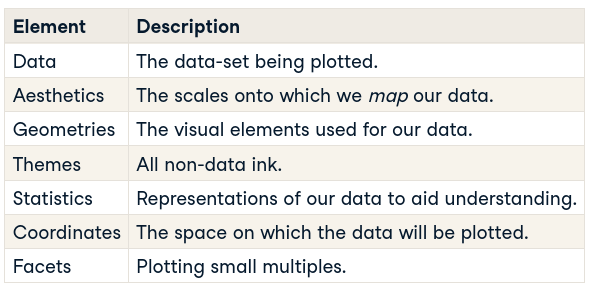
\includegraphics[width=\columnwidth]{img/ggplot.png}
\end{figure}
\begin{figure}[H]
	\centering
	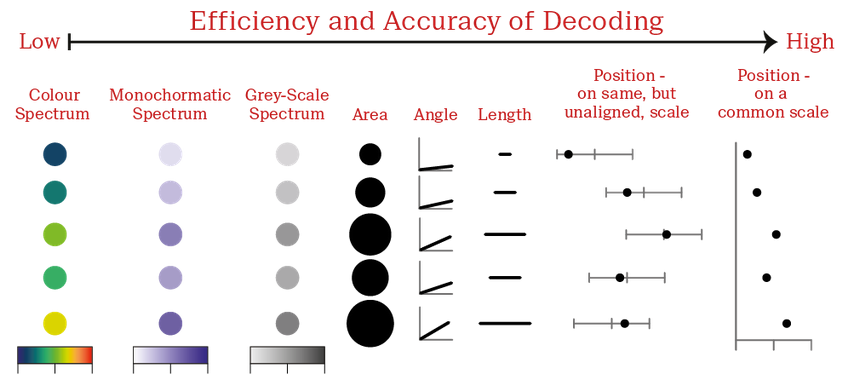
\includegraphics[width=\columnwidth]{img/aes.png}
\end{figure}
\begin{figure}[H]
	\centering
	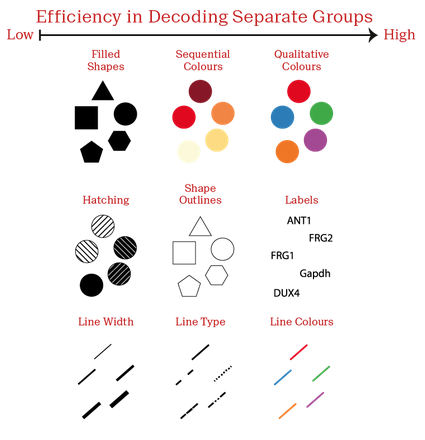
\includegraphics[width=\columnwidth]{img/aes2.png}
\end{figure}

\impt \texttt{vignette("ggplot2-specs")} for help
\begin{lstlisting}[language=R]
ggplot(data = <DATA>) +
    <GEOM_FUNCTION>(mapping = aes(<MAPPINGS>)) + ...
\end{lstlisting}

\begin{itemize}
	\item \underline{Aesthetics}: \texttt{aes(x=..., y=...)}, anything that can change according to the value of the data
	\begin{itemize}
		\item \texttt{size}: to determine size of dots
		\item \texttt{color}: to colour by group
		\item \texttt{alpha}:
		\item \texttt{shape}
	\end{itemize}
    \item \underline{Label}: \texttt{labs()}
    \begin{itemize}
    	\item \texttt{title=}
    	\item \texttt{x=, y=}
    \end{itemize}
    \item \textbf{Types of plot}:
    \begin{itemize}
    	\item \texttt{geom\_point()}: scatter plot
    	\item \texttt{geom\_line()}: line plot
    	\item \texttt{geom\_col()}: barplot
    	\item \texttt{geom\_histogram()}: histogram
    	\item \texttt{geom\_boxplot()}: boxplot
    \end{itemize}
	\item \textbf{Scales}:
	\begin{itemize}
		\item \texttt{scale\_<AES>\_*}: where * is either \texttt{discrete} or \texttt{continuous} or \texttt{manunal}
		\item \texttt{scale\_x\_log10()}: log10 scale
		\begin{itemize}
			\item Alternatively can use \texttt{coord\_trans(x="log10")}
		\end{itemize}
		\item \impt \texttt{scale\_fill\_discrete(name = ..., labels=...)
		\begin{itemize}
			\item name is to change legend title
			\item Labels is to change legend labels
	\end{itemize}}
	\end{itemize}
	\item \texttt{coord\_cartesian}: magnifying glass to expand some areas
	\item \texttt{xlim(), ylim()}: to increase/decrease plotting canvas
	\begin{itemize}
		\item Alternatively can use \texttt{scale\_x\_continuous}
		\item Alternatively can also use \texttt{coord\_cartesian(xlim=c(..., ...))}
	\end{itemize}
    \item \textbf{Aspect ratios}
    \begin{itemize}
    	\item \texttt{coord\_fixed()} to set ratio \texttt{ratio=...}
    \end{itemize}
	\item \textbf{Faceting}:
	\begin{itemize}
		\item \texttt{facet\_wrap(~ ...)}
		\item \texttt{facet\_grid(var1 ~ var2, labeller=...)}
		\begin{itemize}
			\item \texttt{labeller} is for changing the title of each plot
			\item \texttt{fct\_relevel} is to reorder
			\item \texttt{space=...} and \texttt{scales} is to adjust free scales
			\item \texttt{margins=TRUE}: include all points to be plotted in the margins
		\end{itemize}
	\end{itemize}
	\item \texttt{expand\_limits(y=...)}: expand graphing limits
	\item \texttt{coord\_flip()}
	\item \texttt{theme()}
	\item \texttt{labs()}: for labels
\end{itemize}

\subsection{Scatter plot}
\textbf{General pointers}
\begin{itemize}
	\item Is there a general trend/correlation?
	\begin{itemize}
		\item Is it linear?

	\end{itemize}
    \item Who are the ones that \textit{deviate the most} from the trend?
    \item Add more variables (using colour) to investigate the trend
    \item Are there duplicates? check for overplotting?
\end{itemize}
\textbf{Interesting pointers}
\begin{itemize}
	\item If we want to change \texttt{aes} globally, must put the variables outside \texttt{aes(...)} and inside \texttt{geom\_point()}
	\item \texttt{scale\_<AESTHETIC>\_manual}
	\item Discrete colouring vs Continuous colouring? can use \texttt{as.factor()}
	\item to change colour
	\begin{lstlisting}[language=R]
# recommended to use a named vector
cols <- c("8" = "red", "4" = "blue", "6" = "darkgreen", "10" = "orange")
# to change names in legend labels
labs <- c("8" = "Eight", "4" = "Four", "6" = "Six", "10" = "Ten")
scale_colour_mannual(values=cols, labels=labs)\end{lstlisting}
    \item \textbf{Jittering}: points are not plotted at the precise location, but it is useful to solve overplotting
    \begin{lstlisting}[language=R]
geom_point(mapping=..., position="jitter")
geom_point(mapping=..., position=position_jitter(width=0.5, height=0))\end{lstlisting}
    \item \textbf{Nudge position}:
\end{itemize}
\subsection{Histogram}
\textbf{General pointers}
\begin{itemize}
	\item Is it symmetric? or skewed?
	\item Is it bimodal or unimodal??
	\begin{itemize}
		\item If bimodal then might be good to separate the two groups
	\end{itemize}
    \item Outliers (interesting data far away from the norm)
\end{itemize}
\begin{itemize}
	\item \texttt{geom\_histogram()}
	\begin{itemize}
		\item \texttt{bins=...}
		\item \texttt{binwidth=...}
		\item \texttt{boundary=...} to set hard x limit for the histogram
		\item \texttt{col=...}: to control the outline so that it's easy to separate the bin rectangles
	\end{itemize}
	\item \texttt{geom\_freqpoly}: something like histogram but line (similar to cdf plotting)
	\item Aesthetics: \texttt{fill, colour, alpha, x}
	\begin{itemize}
		\item Some computed variables: \impt \texttt{after\_stat} R will compute statistics for each bin, and the value of each bin is then plotted
		\begin{lstlisting}[language=R]
			geom_histogram(aes(x=..., y=after_stat(density)), col=..., fill=...)
			geom_histogram(aes(x=..., y=after_stat(count)), col=..., fill=...)\end{lstlisting}
		\item \texttt{fill=...}: will create two histograms stacked on top of each other
		\item use \texttt{position="dodge"} to prevent stacking
		\item use \texttt{position="identity"} and $\alpha$ to stack histograms on top of another without stacking
		\item \impt we can also use \texttt{position = position\_dodge(arg=...)} to adjust arguments

	\end{itemize}
\end{itemize}

\subsection{Line Plot}
\begin{itemize}
	\item Aesthetic:
	\begin{itemize}
		\item Line type: dashed? dotted?
		\item Line width?
		\item color=....
		\item group= if we want to separate lines but same color
	\end{itemize}
    \item Usually need Tidy Data to separate time series into different groups
    \item \impt \texttt{geom\_area(position="fill")} is interesting
    \item \impt \texttt{geom\_ribbon()} is also interesting
\end{itemize}

\subsection{Geom Text}
\begin{itemize}
	\item \texttt{mapping = aes(x=..., y=..., label=...)}
	\item Usually used in conjunction with \texttt{geom\_line}
\end{itemize}
\subsection{Bar Charts}
\begin{itemize}
	\item \texttt{geom\_col()}: normal bar chart
	\item \texttt{geom\_bar()}: maps count of each category
	\item How to change ordering of bar charts?
	\begin{itemize}
		\item Use \texttt{levels} in \texttt{factor}!
		\item \texttt{reorder()} in mutate!
		\begin{lstlisting}[language=R]
op_budget <- mutate(op+budget, exp_cat = reorder(exp_cat, amount))\end{lstlisting}
	\end{itemize}
\end{itemize}
\begin{lstlisting}[language=R]
ggplot(tv) +
geom_col(mapping=aes(x=year,y=pct, fill=media_activity),
         position="dodge") +
  facet_wrap(~ age) +
  theme(legend.position="bottom")
\end{lstlisting}
\subsubsection{Facet Wrap}
\begin{lstlisting}[language=R]
# to change scale free and wrap labelling
facet_wrap(~ sex, nrow=2, scales="free_x",
           labeller=as_labeller(c('female'="Female", 'male'="Male")))
\end{lstlisting}

\subsection{Smooth Geom}
\begin{itemize}
	\item \texttt{geom\_smooth(aes(...), method="lm")}
	\item \texttt{geom\_smooth(aes(...), method="loess")}
	\item Is the variability around the line the same??
	\item \textbf{Parameters}
	\begin{itemize}
		\item \texttt{span=}: to adjust smoothing
		\item \texttt{se=FALSE}: to remove SE ribbon
	\end{itemize}
\end{itemize}

\subsection{Geom Rug}
\texttt{geom\_rug()}

\subsection{Boxplots}
\begin{itemize}
	\item \impt what to look for: which point/interval has the most common combination!!!
	\item Shows: minimum, 1st quartile, median, 3rd quartile, max values
	\item Also shows outliers (values that lie < 1.5$\times$IQR below the lower quartile or values that lie < 1.5$\times$IQR above the upper quartile)
	\item Useful for identifying outliers, but don't dismiss them so quickly, need to analyze why are there outliers in the first place (are they just following the distribution?)
	\item \impt How to reorder!!!
	\begin{lstlisting}[language=R]
		# order by median
mutate(mpg, class2 = reorder(class, hwy, FUN=median))
\end{lstlisting}
    \item Boxplot secrets
    \begin{lstlisting}[language=R]
# how to find and separate outliers
outliers <- boxplot(mpg$hwy, plot=FALSE)$out

# how to hide outliers
geom_boxplot(outlier.shape=NA)
\end{lstlisting}
\end{itemize}

\subsection{2D-Histograms}
\begin{lstlisting}[language=R]
ggplot(mpg) +
	geom_bin2d(aes(x=displ, y=hwy), binwidth=c(0.5,5)) +
	#scale_fill_gradient(type = "viridis")
	scale_fill_gradient(name="hmm", low="white", high="red")
	# scale_fill_gradientn(colours = terrain.colors(10))
\end{lstlisting}

\subsubsection{Hex bins}
\begin{lstlisting}[language=R]
ggplot(mpg) +
	geom_hex(aes(x=displ, y=hwy), binwidth=c(0.5,5))
\end{lstlisting}

\subsubsection{2D-Density}
\begin{lstlisting}[language=R]
ggplot(mpg) +
	geom_density_2d(aes(x=displ, y=hwy))
\end{lstlisting}
\subsection{2D Heatmaps}
YAYYAYYY
\begin{lstlisting}[language=R]
ggplot(data, mapping=aes(x=displ, y=hwy, z=ma3)) +
	stat_summary_hex(fun=mean, binwidth=c(0.6,5))
\end{lstlisting}
\subsection{Themes}
\begin{itemize}
	\item \impt \texttt{?theme} FOR HELP
	\item \texttt{theme(legend.position = "bottom" OR "none")}
	\begin{itemize}
		\item Alternatively, can position inside the plot where (0,0) represents bottom-left and (1,1) represents top-right
	\end{itemize}
    \item \texttt{axis.ticks}: to remove lines/ticks
    \item \texttt{elements}
    \begin{itemize}
    	\item \texttt{element\_blank()}: to remove shit
    	\item \texttt{<ELE> = element\_<ELE>(args =...)} to adjust arguments
    \end{itemize}
    \item \impt we can also save themes!
    \begin{lstlisting}[language=Java]
t <- theme(...)
ggplot(...) + t
\end{lstlisting}
    \item Import themes
    \begin{itemize}
    	\item theme\_tufte
    	\item theme\_fivethirtyeight
    	\item theme\_wsj
    \end{itemize}
    \item \texttt{theme\_set(t)} to set theme \texttt{t} as default theme

    \item \texttt{panel.grid = NA}: remove grid
    \item \impt \href{https://exts.ggplot2.tidyverse.org/gallery/}{NICE THEMES}
\end{itemize}

\subsection{Grid of Plots (gridExtra)}
\begin{lstlisting}[language=R]
library(gridExtra)
list_of_plots <- list(p1, p2, p3, p4)
grid.arrange(list_of_plots, nrow=2)
\end{lstlisting}

\subsection{Statistics (stats\_)}
\begin{itemize}
	\item \texttt{stat\_count} is basically \texttt{geom\_bar}
	\item \texttt{stat\_bin} is basically \texttt{geom\_histogram}
	\item \texttt{stat\_smooth} is basically \texttt{geom\_smooth}
	\item \texttt{stat\_summary} is for confidence intervals?
	\begin{lstlisting}[language=R]
ggplot(iris, aes(x=Species, y=Sepal.Length)) +
  stat_summary(fun.data = mean_sdl,
               fun.args = list(mult=1), # 1 standard deviation
               geom="errorbar",
               width=0.1)
	\end{lstlisting}
    \item \impt QQ plot
    \begin{lstlisting}[language=R]
iris %>%
  ggplot(aes(sample=Sepal.Length)) +
  stat_qq() +
  geom_qq_line(col="red")
\end{lstlisting}
\end{itemize}

\section{Exploratory Data Analysis (EDA)}
\subsection{Exploration}
\begin{quote}
	The greatest value of a picture is when it forces us to notice what we never expected to see
\end{quote}
\textbf{Process}
\begin{itemize}
	\item Generate questions about our data
	\begin{itemize}
		\item What type of variation occurs within my variables?
		\item What type of covariation occurs between my variables?
		\item Which values are the most common? Why?
		\item Which values are rare?
		\item Are there any unusual patterns in the data?
	\end{itemize}
	\item Search for answers by visualizing, transforming, and modelling our data
	\item Use what we learn to refine our questions and/or generate new questions (technical knowledge)
	\item Audience? is it for a tech/non-technical audience?
\end{itemize}

\subsubsection{Contingency Table}
\begin{itemize}
	\item Let $A$ and $B$ be two groups with each of them having $E$ or $E^C$, we want to compute the proportions of $E$ within the groups $p_A$ and $p_B$
	\item $p_A$ is estimated by $\hat{p_A}$, likewise $\hat{p_B}$
	\item Is the difference of $p$ between the two groups significant? in other words, \underline{is there any association} between the group and event $E$?
	\begin{itemize}
		\item Difference of proportion: $\hat{p}_1 - \hat{p}_2$
		\item Relative risk: $\hat{p}_1/\hat{p}_2$
		\item Let $p$ be the probability of success, and $1-p$ be the probability of failure
		$$\text{odds} = \frac{p}{1-p} \in [0,\infty)$$
		\item Log-odds ratio: ratio of log odds
	\end{itemize}
    \item Within different groups, are the distribution/pmf the same?
    \begin{figure}[H]
    	\centering
    	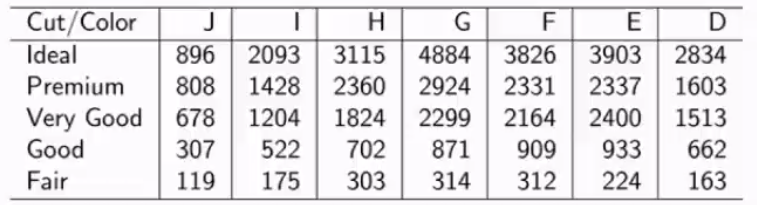
\includegraphics[width=\columnwidth]{img/contingency.png}
    \end{figure}
    \item \impt \texttt{geom\_mosaic}!
    \begin{lstlisting}[language=R]
library(ggmosaic)
ggplot(diamonds) +
  geom_mosaic(aes(x=product(color), fill=cut))
\end{lstlisting}
    \item Assuming independence,
    $$\Pr(AB) = \Pr(A)\Pr(B)$$
    but this is not always true, so can calculate the probability of each column/row and compare with the real table
    \begin{itemize}
    	\item Deviation from independence tells us about association!
    	\begin{lstlisting}[language=R]
library(GGally)
ggtable(d, "color", "cut",
        cells="col.prop",
        fill="std.res")
\end{lstlisting}
    \end{itemize}
\end{itemize}

\subsection{Colours}
\begin{lstlisting}[language=R]
# table/heatmaps
diamonds %>%
  mutate(mean_price_cat = cut(mean_price, c(2000, 3000, 5000, 8000))) %>%
  ggplot() +
  geom_tile(aes(x=color, y=cut, fill=mean_price_cat)) +
  geom_text(aes(x=color, y=cut, label=round(mean_price,0))) +
  scale_fill_brewer(palette="YlOrRd")
\end{lstlisting}
\begin{itemize}
	\item Different hues: different groups
	\item Different value: good for ordering
	\item \texttt{scale\_fill\_gradientn} or \texttt{scale\_fill\_gradient2}
	\item Example:
	\begin{lstlisting}[language=R]
scale_fill_gradient2(low="red", mid="white", high="blue", midpoint=5000)
\end{lstlisting}
    \item \texttt{RColorBrewer} package
    \begin{lstlisting}[language=R]
?brewer.pal
display.brewer.all()
\end{lstlisting}
\end{itemize}

\subsection{Correlation Matrices}
\begin{itemize}
	\item \texttt{Hmisc::describe()}
	\item Info correlates to how much information the variable is giving, higher info means more useful
	\item Gmd is Gini's mean difference to measure dispersion
	\begin{lstlisting}[language=R]
cor_Cars93 <- select(Cars93, which(!sapply(Cars93, is.factor))) %>%
cor(. , use="pair")
# need to convert to tidy data format to plot correlation matrix
cor_Cars93_df <- as.data.frame(cor=Cars93, row.names=NULL) %>%
                 mutate(var1=row.names(cor_Cars93)) %>%
                 pivot_longer(Min.Price:Weight, names_to="var2", values_to="correlation")
\end{lstlisting}
\end{itemize}
\subsection{Hierarchical Clustering}
\textbf{Definition}: identify groups within the data, such that members within a group are "similar" to one another
\begin{itemize}
	\item We can cluster variables (the columns) or the observations (rows)
\end{itemize}
\subsubsection{Dissimilarity Measures}
\textbf{Between individual observations}: $d$ measures pairwise dissimilarity between individual observations (distance?)
\begin{itemize}
	\item Euclidean distance is the most common choice
	$$d(x_i,x_j) = \sum_{s=1}^p(x_{is}-x_{js})^2$$
	\item $L1$-norm
	$$d(x_i,x_j) = \sum_{s=1}^p|x_{is}-x_{js}|$$
\end{itemize}
\textbf{Between groups}: not just between individual points, we also need to generalize dissimilarity/similarity between groups of observations
\begin{itemize}
	\item \underline{Single linkage}: dissimilarity is the closest (least dissimilar) pair
	$$d_S(G,H) = \min_{i\in G,j\in H}d(x_i,x_j)$$
	\item \underline{Complete linkage}: dissimilarity is the furthest (most dissimilar) pair
	$$d_C(G,H) = \max_{i\in G,j\in H}d(x_i,x_j)$$
	\item \underline{Average linkage}: the average of all pairwise dissimilarities between the groups
	$$d_A(G,H) = \frac{1}{N_GN_H}\sum_{i\in G}\sum_{j\in H}d(x_i,x_j)$$
	\item \underline{Ward linkage}: returns more compact clusters
\end{itemize}
\textbf{Algorithm}
\begin{enumerate}
	\item Assume we start with $n$ observations
	\item Get pairwise distances between observations, store it in a $n\times n$ matrix
	\begin{itemize}
		\item In our case the dissimilarity measure is
		$$d(v_1,v_2)=\frac{1-\text{cor}(v_1,v_2)}{2}, 0\leq d(v_1,v_2)\leq1$$
	\end{itemize}
	\item get the minimum dissimilarity measure (distance) in the matrix, and group the two observations together
	\item Return a $(n-1)\times (n-1)$ matrix where the two observations are grouped
	\item Repeat until we have 1$\times$1 matrix

\end{enumerate}
\textbf{Dendrogram}
\begin{itemize}
	\item The height is the dissimilarity measure between the two child nodes
	\item Cut the tree horizontally and get groupings
	\begin{lstlisting}[language=R]
#split into 5 grps
as.factor(cutree(hc,k=5))
\end{lstlisting}
\end{itemize}
\begin{lstlisting}[language=R]
# cor_Cars93_df is from section 9.3
## the disimilarity measure used here is (1-correlation)/2
hc <- hclust(as.dist((1-cor_mtcars)/2))
plot(as.dendrogram(hc))

# ordering for plot
ord <- order.dendrogram(as.dendrogram(hc))

cor_Cars93_df2 <- mutate(cor_Cars93_df,
                 var1=factor(var1, levels=row.names(cor_Cars93)[ord]),
                 var2=factor(var2,
                 levels=row.names(cor_Cars93)[ord]))

ggplot(cor_Cars94_df2) +
geom_tile(aes(x=var1, y=var2, fill=correlation))  +
scale_fill_gradient2() +
theme(axis.text.x=element_text(angle=90,vjust=0,hjust=1))
\end{lstlisting}
\subsection{Multidimensional Scaling}
\begin{itemize}
	\item To visualize similarities of high-dimensional data
	\item With a choice of $k$ (number of dimensions?), we seek values $z_1,z_2,\dots,z_N\in\mathbb{R}^k$ such that the following function is minimised
	$$S(z_1,\dots z_N) = \left[\sum_{i\neq j}(d(x_i,x_j)-||z_i-z_j||)^2\right]^{1/2}$$
\end{itemize}
\begin{lstlisting}[language=R]
cars_dist <- as.dist((1-cor_Cars93)/2)
mds2 <- MASS::sammon(cars_dist, k=2)
grps <- as.factor(cutree(hc,k=5))
mds_df <- data.frame(mds2$points) %>%
  mutate(label=row.names(mds2$points),Cluster=grps) %>%
  rename('Var.1' = 'X1', 'Var.2' = 'X2')
# then plot the data with reduced dimension with all the colouring
\end{lstlisting}

\section{Interesting stuff}
\begin{itemize}
	\item Can lookup location through zipcode
	\item \textbf{Which geom to use?}
	\begin{itemize}
		\item What is the question? if no question, just pick two variables
		\item Inspect types of variables
		\item Who is your viewer/audience?
		\item Do I need to add another variable?
		\item Do we need to transform/bin the data differently?
		\item Do we need to add a smooth?
		\item Why are there so many outliers?
		\item Do they follow some patterns that could be explained by another variable?
	\end{itemize}
    \item \impt \texttt{library(GGally)}: for correlation plot, useful for EDA
    \begin{lstlisting}[language=R]
# create correlation plot
ggpairs(data)
\end{lstlisting}
    \item \texttt{library(plotly)}: for interactive plot
\end{itemize}

\section{Data Cleaning}
\begin{itemize}
	\item Duplicate rows (use id to clean)
	\item NA values
\end{itemize}
\end{multicols}






\end{document}